\documentclass[12pt,a4paper]{article}
\usepackage[utf8]{inputenc}
\usepackage[spanish]{babel}
\usepackage{amsmath}
\usepackage{amsfonts}
\usepackage{amssymb}
\usepackage{geometry}
\usepackage{listings}
\usepackage{xcolor}
\usepackage{graphicx}
\usepackage{float}
\geometry{margin=2.5cm}

% Configuración de listings para código R
\lstset{
    basicstyle=\ttfamily\small,
    breaklines=true,
    breakatwhitespace=true,
    frame=single,
    language=R,
    showstringspaces=false,
    columns=flexible
}

\title{Estadística y Diseño de Experimentos\\
Ejercicios 1}
\date{11 de Junio, 2025}
\author{}

\begin{document}

\maketitle

\noindent\textbf{Nombre del alumnx:} \underline{\hspace{0.5cm}Martínez Buenrostro Jorge Rafael\hspace{0.5cm}}

\vspace{1cm}

\begin{itemize}
\item Considere los siguientes datos:

\begin{center}
6,4 8,1 4,7 8,7 4,6 7,9 4,1 7,9 2,8 8,8 7,0 7,0 3,5 8,7 4,1
\end{center}

Para ingresar los datos en R, puede usar el siguiente comando:
\begin{lstlisting}
datos <- c(6.4, 8.1, 4.7, 8.7, 4.6, 7.9, 4.1, 7.9, 2.8, 8.8, 7.0, 7.0, 3.5, 8.7, 4.1)
\end{lstlisting}

\begin{enumerate}
\item Calcule la media muestral
Para calcular la media muestral en R, puede usar el siguiente comando:
\begin{lstlisting}
    mean(datos)
\end{lstlisting}
Lo que nos da como resultado: \(\bar{x} = 6.286667\)
\vspace{1cm}

\item Calcule la varianza muestral
Para calcular la varianza muestral en R, puede usar el siguiente comando:
\begin{lstlisting}
    var(datos)
\end{lstlisting}
Lo que nos da como resultado: \(s^2 = 4.452667\)
\vspace{1cm}

\item Encuentre los cuartiles $Q_1$, $Q_2$ y $Q_3$
Para calcular los cuartiles en R, puede usar el siguiente comando:
\begin{lstlisting}
    quantile(datos, probs = c(0.25, 0.5, 0.75))
\end{lstlisting}
Lo que nos da como resultado: \(Q_1 = 4.35\), \(Q_2 = 7.00\), \(Q_3 = 8.00\)
\vspace{1cm}

\item Grafique el histograma para estos datos. Para graficar el histograma en R, puede usar el siguiente comando:
\begin{lstlisting}
    hist(datos, main = "Histograma de los datos", xlab = "Valores", ylab = "Frecuencia", col = "lightblue")
\end{lstlisting}
Lo que nos da el siguiente histograma:
\begin{figure}[H]
    \centering
    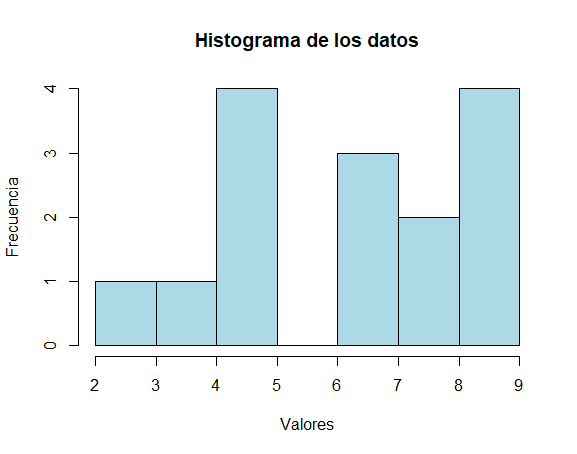
\includegraphics[width=0.7\textwidth]{img/Histograma.png}
\end{figure}
¿Parecen provenir de una distribución normal? Basándose en el histograma, los datos no parecen provenir de una distribución normal.

\vfill

\item Grafique el diagrama de caja y brazos. Para graficar el diagrama de caja y brazos en R, puede usar el siguiente comando:
\begin{lstlisting}
    boxplot(datos, main = "Diagrama de Caja y Brazos", ylab = "Valores", col = "lightgreen")
\end{lstlisting}
Lo que nos da el siguiente diagrama de caja y brazos:
\begin{figure}[H]
    \centering
    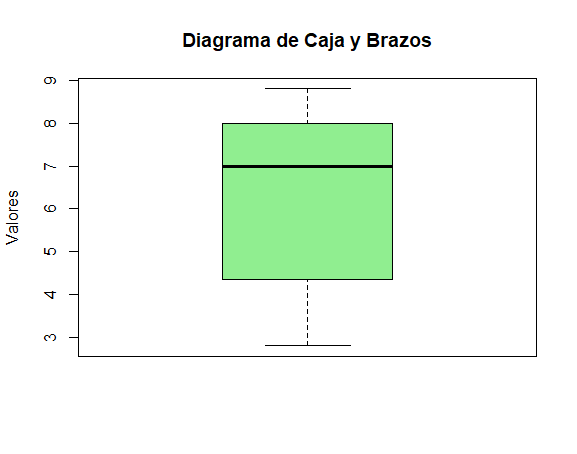
\includegraphics[width=0.7\textwidth]{img/DiagramaCajas.png}
\end{figure}
¿Qué puede decir sobre la variabilidad de los datos? Los datos presentan una alta variabilidad, ya que el rango intercuartílico va de aproximinadamente 4.35 a 8.0. Muestra que el 50\% central de los datos está bastante disperso.

\end{enumerate}

\end{itemize}

\end{document}